%!TeX root=../tese.tex
%("dica" para o editor de texto: este arquivo é parte de um documento maior)
% para saber mais: https://tex.stackexchange.com/q/78101/183146

%% ------------------------------------------------------------------------- %%
\chapter{Balanceamento Dinâmico}
\label{cap:balanceamento dinamico}
\section{Conceito de Interpretação}

Com o objetivo de medir a dificuldade de um jogo e parametrizá-la em uma ou mais variáveis utilizáveis pelo desenvolvedor, é proposta a divisão da experiência geral do jogo em desafios menores e separados, para realização, assim, da medição da dificuldade de cada um destes desafios, assim como realizado por \citet{ExperimentalValidation}. Aponte propõe que a interpretação de \emph{um desafio} como \emph{o objetivo de obter um determinado resultado} permite a extração de um conjunto de desafios que compoem a experiência de jogo apresentada ao jogador.

Com isso, ao medir a dificuldade de tais desafios que compoem o jogo, torna-se possível medir a dificuldade geral do jogo em questão. Estes desafios menores podem derivar tanto de elementos gerados dinamicamente, quanto estaticamente, como por exemplo fases e inimigos descritos em um banco de dados, método usado neste estudo.

\section{Habilidades e Desafios Medidos}

Independente da origem de um desafio em um determinado estado do jogo, o sistema implementado sempre interpretará as ações do jogador em intervalos de tempo em termos de \textit{sucesso} ou \textit{falha}. Essa separação torna-se necessária para o uso de uma heurística para aproximação da dificuldade dos desafios. Tendo essas duas opções em mente, a dificuldade de um desafio é estimada pela probabilidade do jogador \textit{falhar} em concluir tal desafio com sucesso. Além disso, é importante pensar também na variação contínua de dificuldade por parte das habilidades do jogador. Conforme este se adapta aos desafios, sua habilidade cresce, e portanto a sua probabilidade de falhar os desafios diminui. Com isso, os desafios e suas recompensas devem crescer de acordo. Estes conceitos e suas abordagens de implementação serão aprofundados ainda neste capítulo.

Em favor da simplicidade, os desafios são ainda separados em categorias menores, denominadas \textit{tarefas simples} e \textit{tarefas compostas} por \citet{ExperimentalValidation} e \citet{FearOfFailing}. \textit{Tarefas simples} representam as ações mais simples possíveis do jogo, como movimentação, ataques, desvios, bloqueios, entre outras, por isso tendem a ser repetidas diversas vezes em um curto período de tempo. \textit{Tarefas compostas} tendem a consumir mais tempo, diversas ações, e serem relativamente únicas, como a tarefa de derrotar um inimigo qualquer, derrotar um chefe, sobreviver uma onda de inimigos, ou até mesmo completar o jogo.

Como as tarefas simples tendem a ser apresentadas diversas vezes para o jogador, estas não proporcionarão uma recompensa tão considerável quanto a de tarefas compostas, uma vez que a habilidade do jogador não mudará de forma drástica o suficiente para tal. Por outro lado, tarefas compostas apresentarão uma recompensa maior, assim como também estarão sucetíveis a variações de recompensa maiores entre suas conclusões.

Para cada tarefa, é necessário definir uma ação de conclusão e uma condição de recompensa. Por exemplo, o jogador terá constantemente a tarefa de \textit{não ser atingido por balas inimigas}. Isso é, para cada bala inimiga que o jogador não for atingido, ele receberá uma recompensa, neste caso, pequena, pelo fato deste frequentemente enfrentar múltiplas balas simultaneamente. Caso falhe em concluir a tarefa (seja atingido), o jogador é punido (perde uma vida) e a dificuldade geral do jogo é diminuída de acordo.

\section{Aplicação no Protótipo}

\subsection{Leitura}

Neste estudo, o cálculo da dificuldade se baseou na seguinte divisão de ações/tarefas do jogador:

\begin{itemize}
    \item Pontos de dano;
    \item Pontos de \textit{graze}.
\end{itemize}

\textit{Graze}, terminologia utilizada na saga \textit{Touhou}~\citep{Touhou}, denomina a ação de passar os mais próximo possível de uma bala inimiga com o a \textit{hitbox} do personagem, em um \textit{Shmup}, literalmente \textquotedbl{raspando}\textquotedbl{} próximo à bala.

Os pontos de dano são calculados considerando o tempo total desde que o jogador entrou em contato com uma bala inimiga e quantas balas inimigas estão ativas na tela no momento, da seguinte maneira:

$$
no\_hit\_points = \frac{no\_hit\_time^{1.15} * n\_bullets}{500}
$$

onde $no\_hit\_time$ representa o tempo, em segundos, desde a última colisão do jogador com uma bala inimiga, e $n\_bullets$, o número de balas inimigas na tela no momento. Este valor é apenas considerado quando existem inimigos ativos no momento.

Os pontos de \textit{graze}, por sua vez, são calculados da seguinte maneira:

$$
graze\_points = grazed\_bullets * (overall\_difficulty + 1)^{0.2}
$$

onde $grazed\_bullets$ é o número de balas \textquotedbl{raspadas}\textquotedbl{} desde o último cálculo de dificuldade. Após o cálculo, $grazed\_bullets$ é zerado. $overall\_difficulty$ é a dificuldade total atual, calculada da maneira a seguir:

$$
overall\_difficulty = overall\_difficulty + \frac{no\_hit\_points + graze\_points}{2}
$$\label{overallDiffCalc}

tendo $overall\_difficulty$ inicializada com 0. O método a seguir, realizador do cálculo, é definido no \textit{script} da fase e chamado pelo personagem apenas a cada meio segundo, a fim de evitar inflação de valores e otimizar o tempo de processamento.

\begin{programruledcaption}{Função principal de cáulculo da dificuldade\label{prog:diff_calc}.}
    \begin{lstlisting}[
        language=Python,
        style=wider,
        functions={},
        specialidentifiers={},
    ]
        func update_diff(no_hit_time, grazed_bullets):
            var core_action_points = 0
            
            var no_hit_points = 0
            var graze_points = 0
            
            # Points gained from not getting hit, considering time and amount of
            # bullets on screen
            no_hit_points = pow(no_hit_time, 1.15) * n_bullets / 500
            graze_points = grazed_bullets * pow(overall_difficulty + 1, 0.2)

            core_action_points = no_hit_points + graze_points
            
            var accumulated_diff = core_action_points / 2
            overall_difficulty += accumulated_diff

            stats.update_diff(accumulated_diff, overall_difficulty)
            
            for enemy in $Enemies.get_children():
                for generator in enemy.get_node("Generators").get_children():
                    generator.update_diff(overall_difficulty)
    \end{lstlisting}
\end{programruledcaption}

Nas últimas 3 linhas do código, é feita a atualização de parâmetros dentro dos inimigos, sendo assim, a aplicação da dificuldade no ambiente do jogo.

\subsection{Alteração de Inimigos}

Os cálculos realizados acima são então interpretados pela classe de \textit{gerador de balas} dos inimigos. O \textit{gerador de balas} (ou apenas \textit{gerador}) genérico é uma cena dedicada à criação de projéteis por parte dos inimigos. Esta foi desenvolvida para receber uma gama de atributos definidores do comportamento dos ataques do inimigo. Cada inimigo pode ter um número de geradores maior ou igual a zero. Alguns dos atributos do gerador seguem:

\begin{itemize}
    \item $proj\_type$: Tipo de projétil a ser disparado;
    \item $life$: Tempo de vida de cada projétil gerado;
    \item $bullets\_per\_array$: Número de projéteis por \textit{vetor} de projéteis;
    \item $individual\_array\_spread$: Ângulo formado por cada um dos vetores;
    \item $total\_bullet\_arrays$: Número de projéteis em cada vetor;
    \item $base\_spin\_speed$: Velocidade de rotação do gerador;
    \item $spin\_variation$: Variação da velocidade de rotação (aceleração de rotação);
    \item $aim\_at\_character$: \textit{Flag} definindo se os vetores se direcionarão automáticamente à posição do personagem, ignorando a rotação do gerador;
    \item $bullet\_speed$: Velocidade dos projéteis;
    \item $fire\_rate$: Frequência na qual os projéteis são disparados;
\end{itemize}

Por exemplo, um \textit{vetor} com 3 projéteis e $90^{\circ}$ de abertura resultará em 3 balas com $45^{\circ}$ de inclinação entre si, saindo do ponto de origem do gerador. A imagem a seguir mostra dois inimigos no topo da tela, ambos com um único vetor com abertura de $25^{\circ}$, porém o inimigo da direita com 3 projéteis por vetor, resultando em um projétil a mais no centro da abertura. Uma classe de exemplo e testes de geradores pode ser encontrada no apêndice \ref{ap:generator demo}.

\begin{figure}
    \centering

    \begin{subfigure}{.7\textwidth}
        \centering
        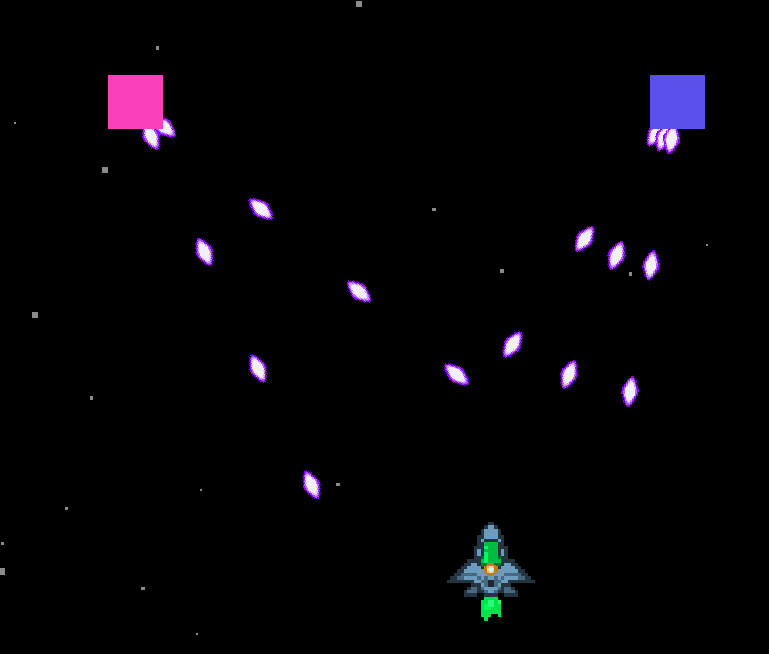
\includegraphics[width=1\textwidth]{geradores1}
    \end{subfigure}

    \caption{Exemplo de geradores com projéteis (em roxo) focados no personagem.}
\end{figure}

Estes dados são carregados sempre do banco de dados (\ref{BancoDeDados}) para inicialização dos inimigos. Estes valores, porém, não serão sempre os mesmos para os inimigos. Conforme a variável $overall\_difficulty$ é alterada~(\ref{overallDiffCalc}), modificadores para estes valores são calculados dentro dos inimigos também, processo executado nas 3 últimas linhas do programa \ref{prog:diff_calc}. Nisso, as seguintes variáveis são calculadas.\\
\\
$mod\_bullet\_speed = overall\_difficulty^{0.05} - 1$\\
$mod\_spin\_speed = ???$\\
$mod\_fire\_rate = log_{10} overall\_difficulty$\\
$mod\_bullets\_per\_array =  \begin{cases}
                                0,& \text{se } overall\_difficulty< 50\\
                                1,              & \text{caso contrário}
                            \end{cases}$\\
\\
e, com isso, os valores do gerador são alterados da seguinte maneira, quando considerados na instanciação de projéteis.\\
\\
$bullet\_speed = mod\_bullet\_speed + bullet\_speed$\\
$spin\_speed = mod\_spin\_speed * spin\_speed$\\
$fire\_rate = mod\_fire\_rate * fire\_rate$\\
$bullets\_per\_array = mod\_bullets\_per\_array + bullets\_per\_array$

aaaaaa


